\section{Resultados}
Despues de procesar los resultados del experimento el script the python nos arrojo las siguientes graficas:
\begin{figure}[H]
    \centering   
    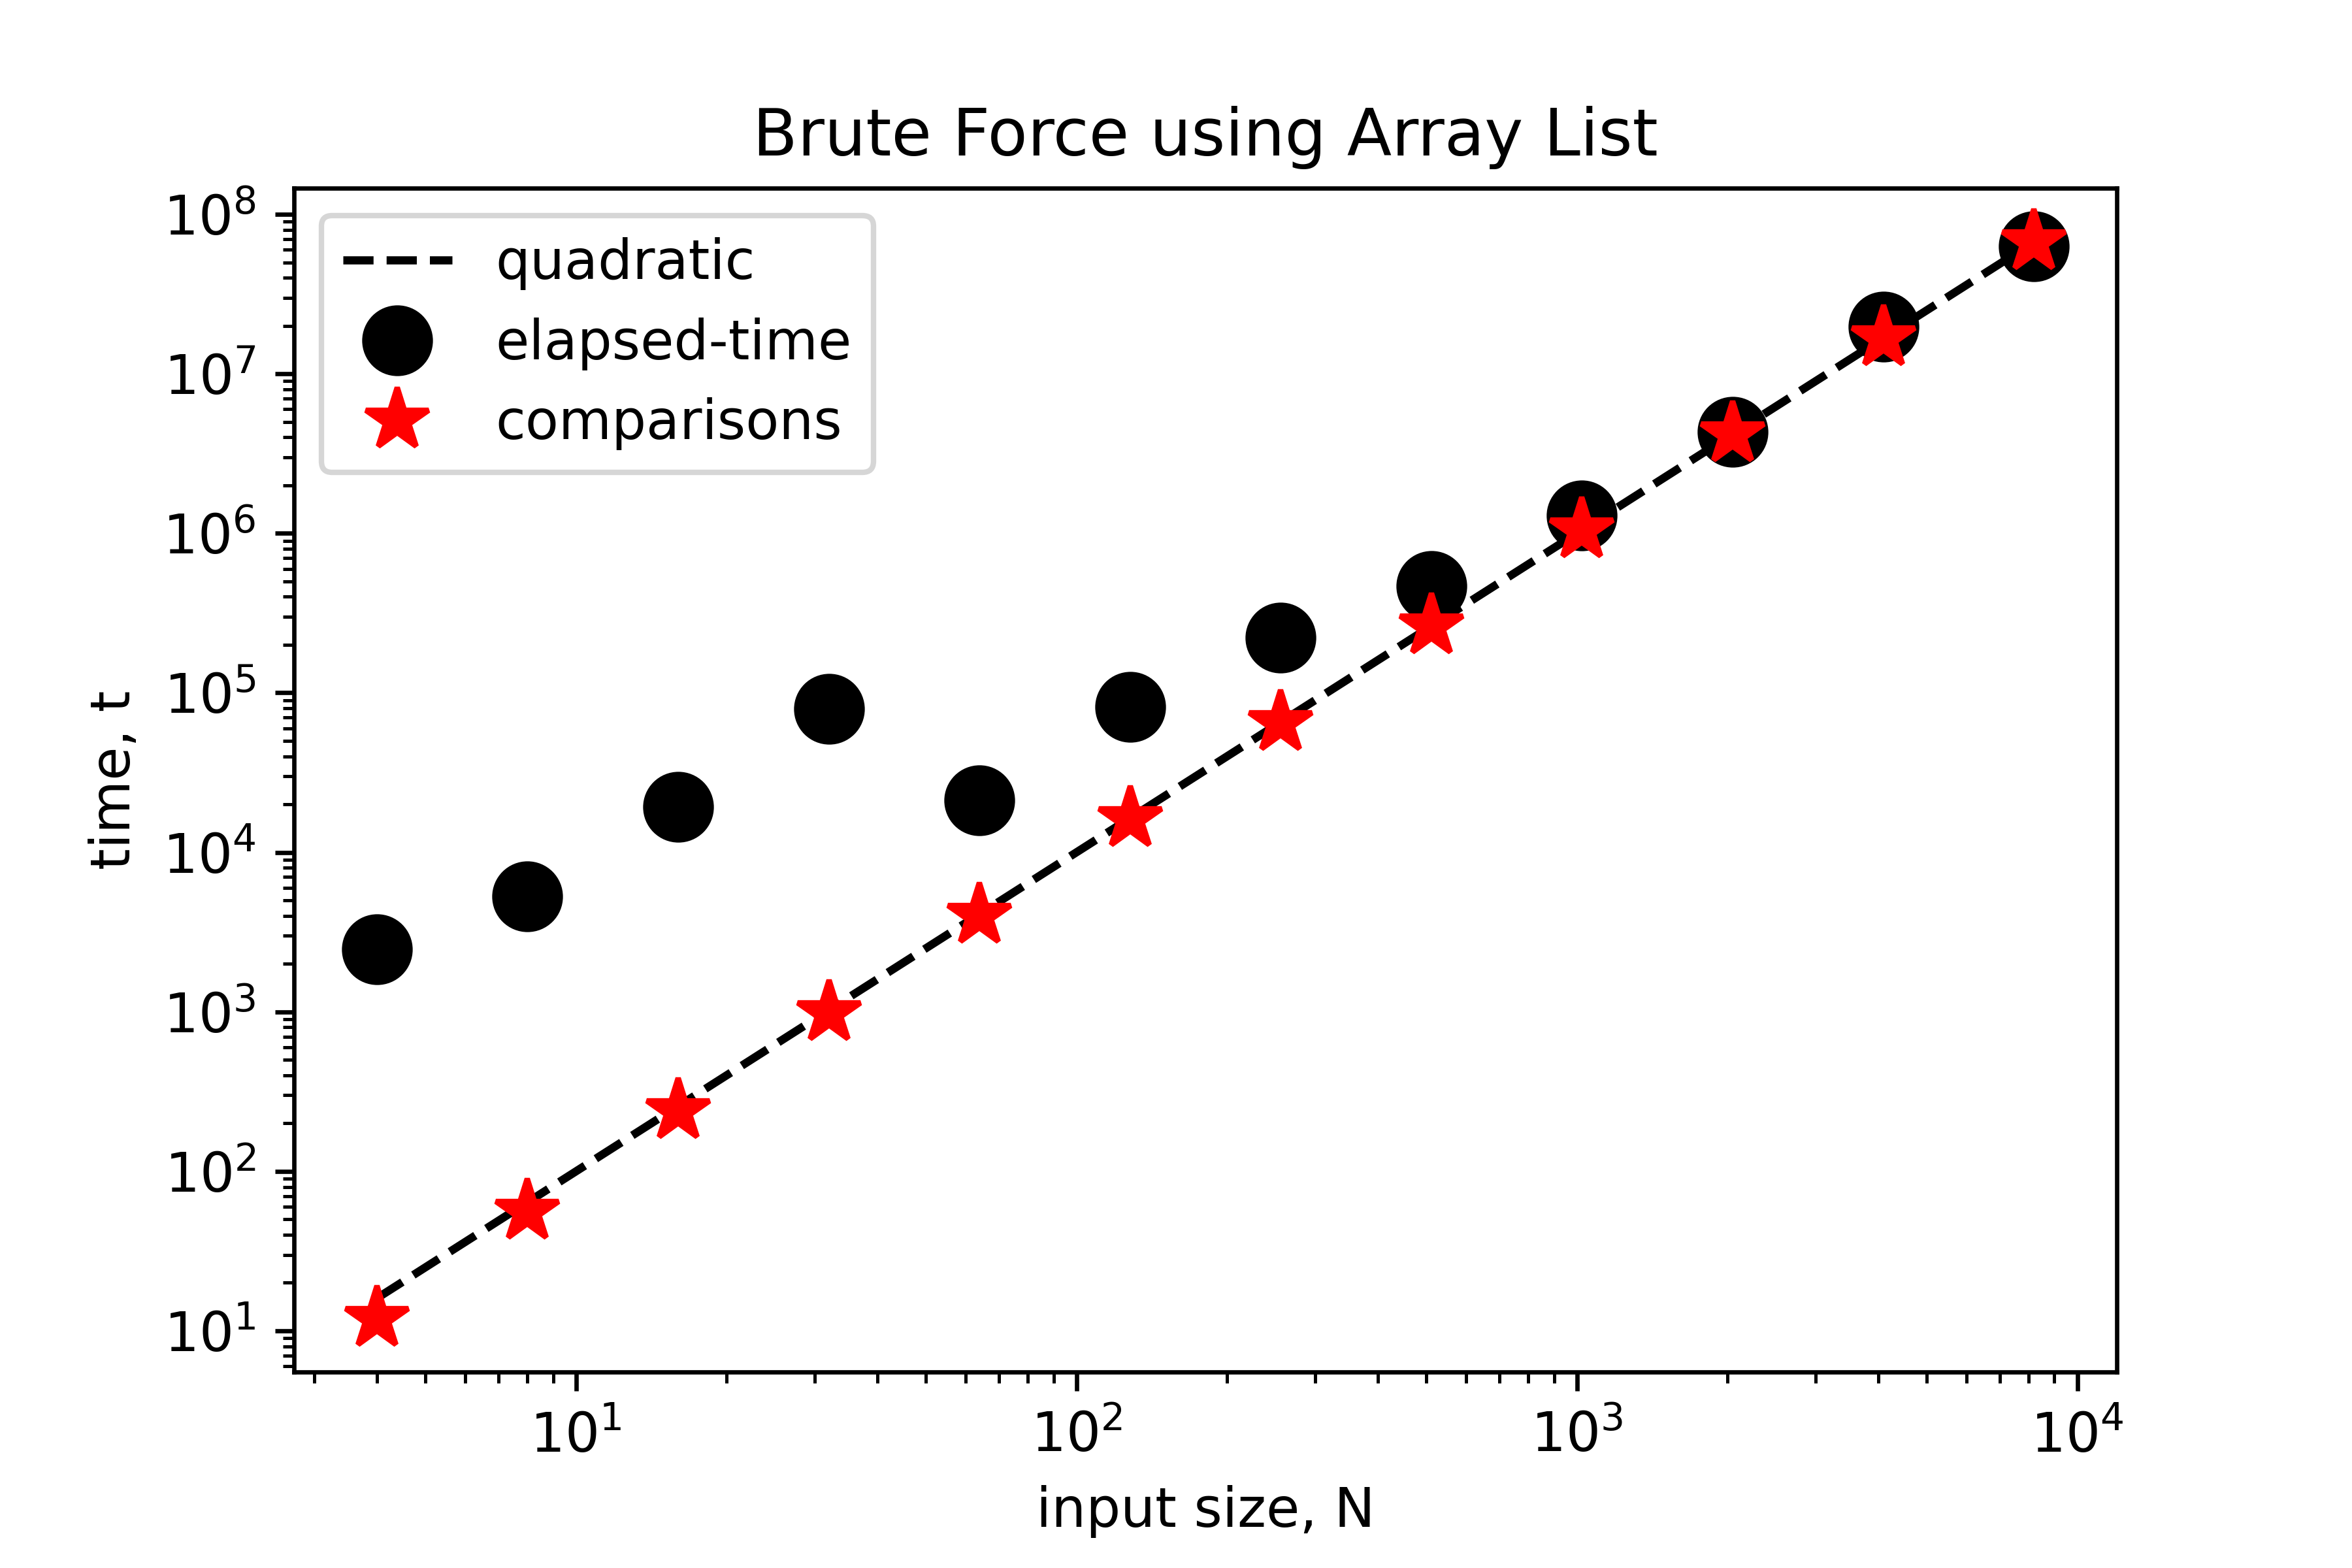
\includegraphics[width=0.45\textwidth,\keepaspectratio]{Images/BruteArray.png}
    \caption{Comportamiento de la tecnica de \textit{Fuerza Bruta} usando \textit{Array Lists}}
\end{figure}%

\begin{figure}[H]
    \centering    
    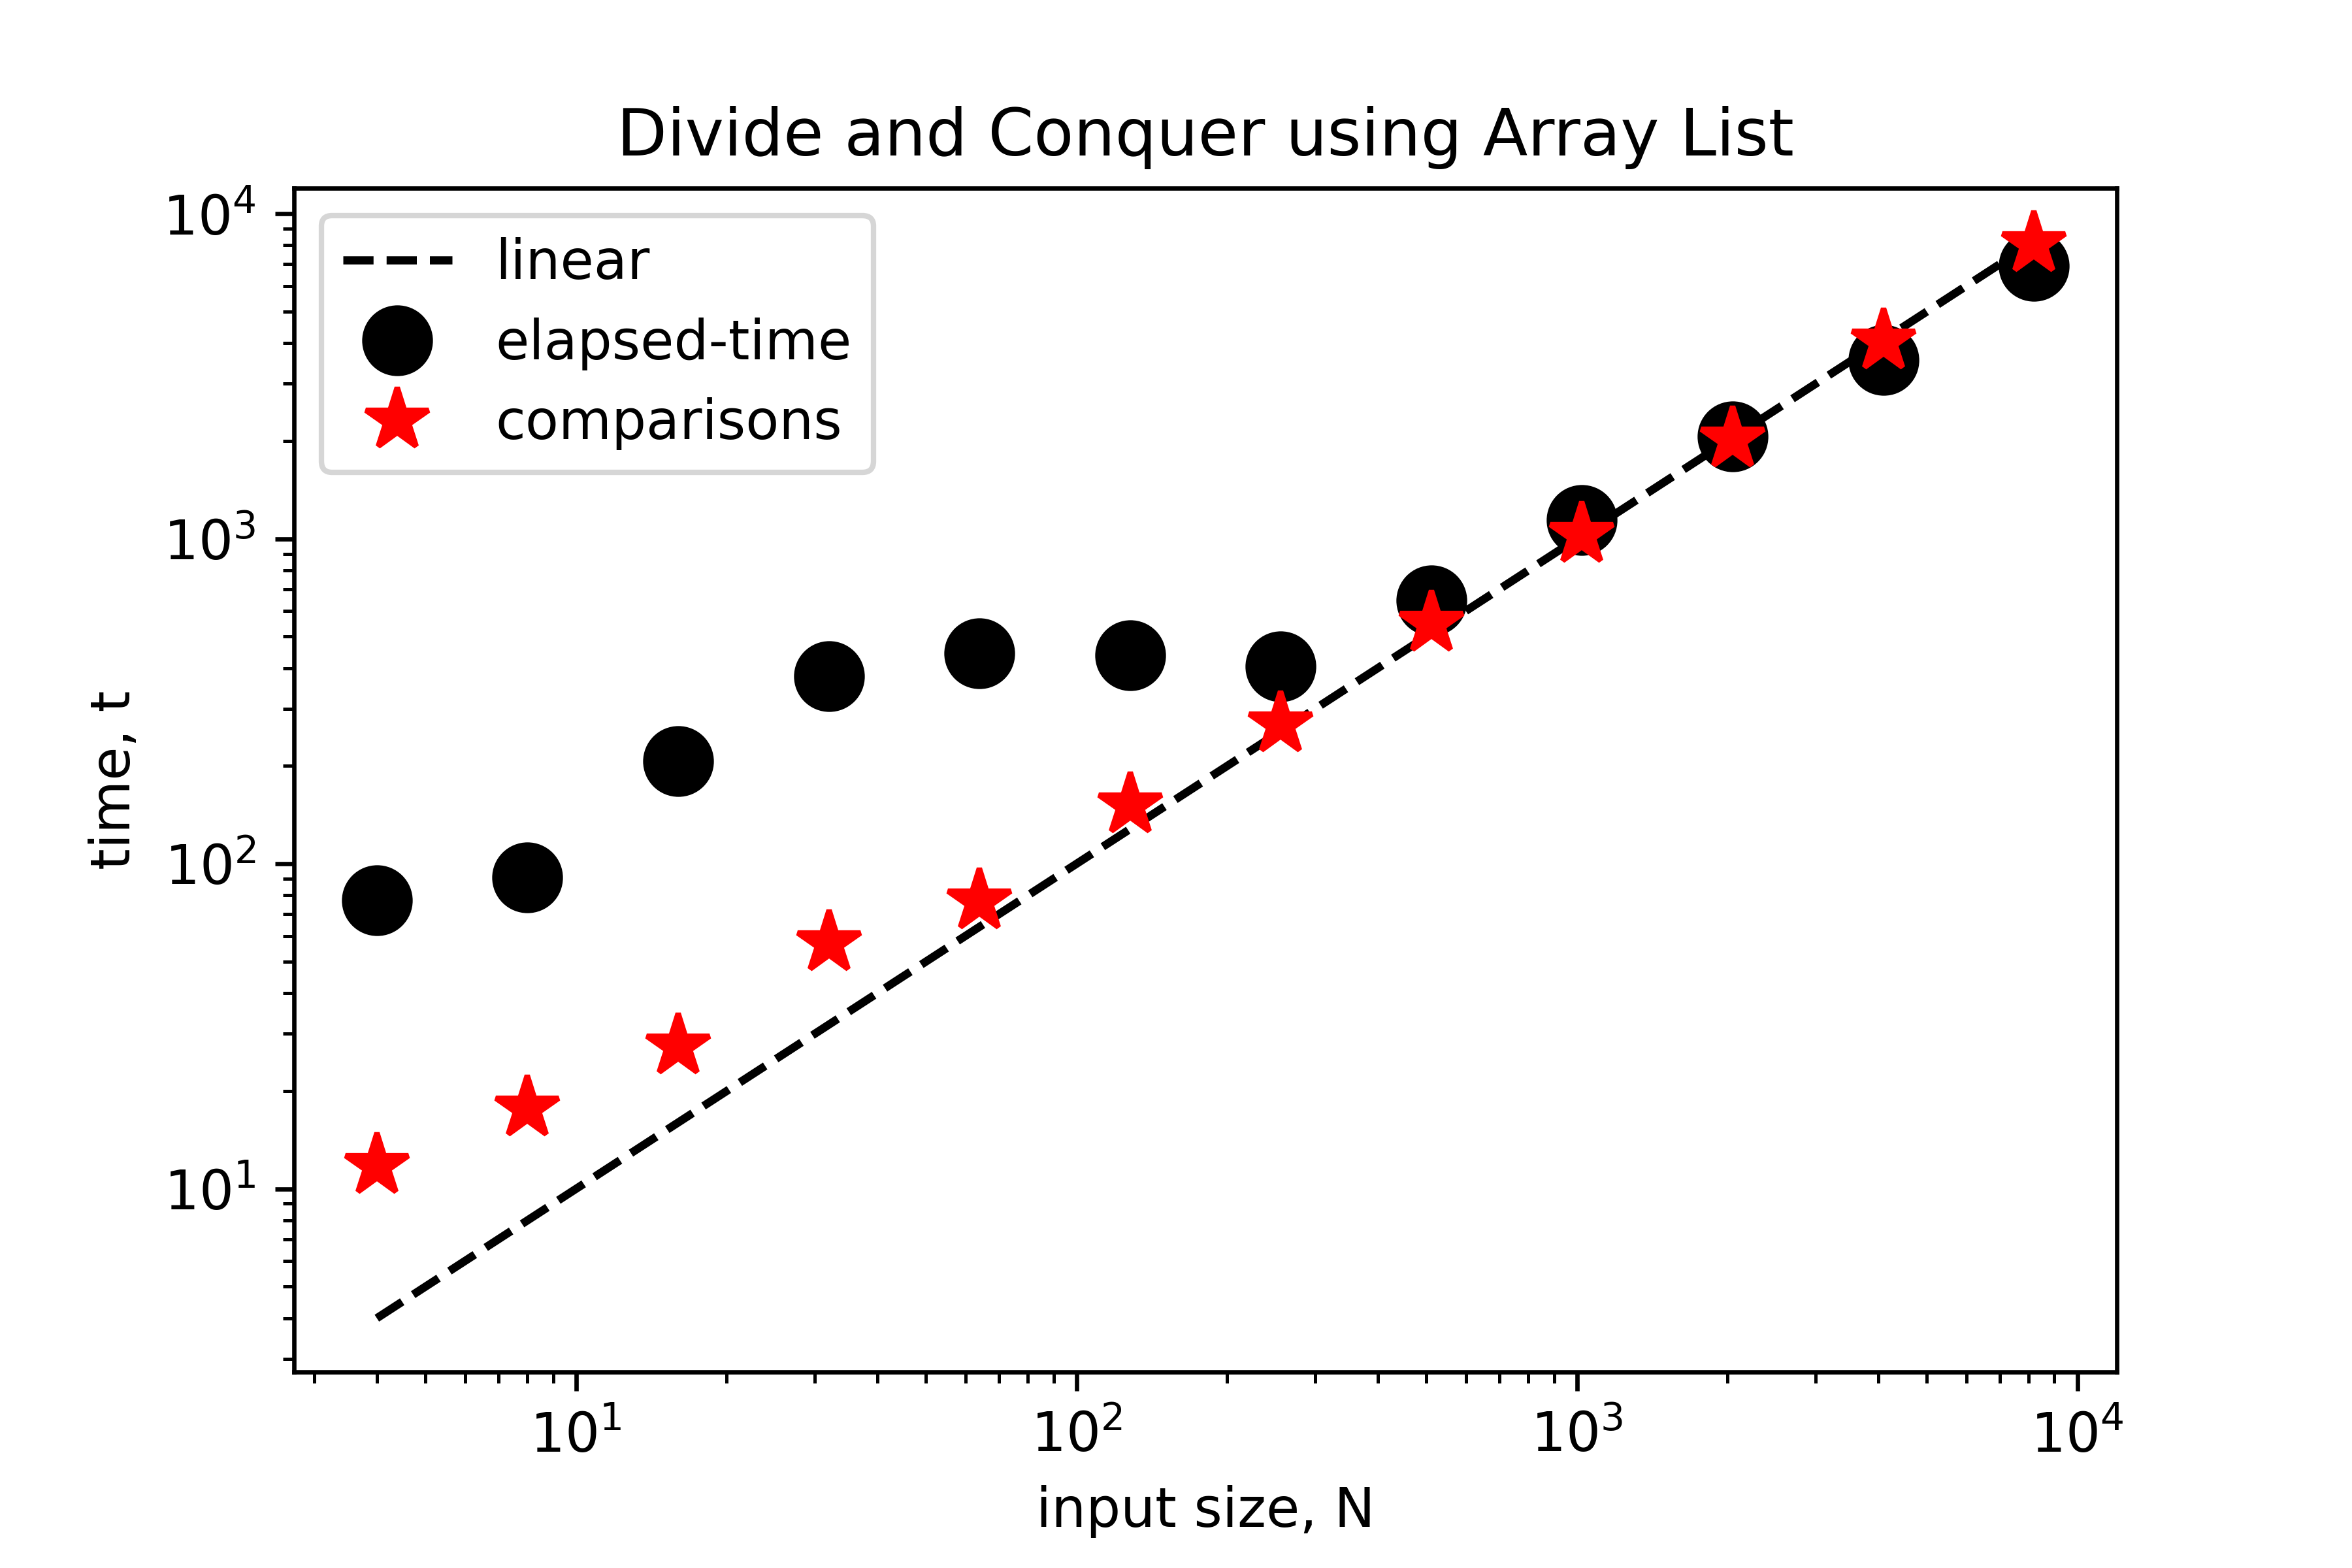
\includegraphics[width=0.45\textwidth,\keepaspectratio]{Images/DivideArray.png}
    \caption{Comportamiento de la tecnica de \textit{Divide y Venceras} usando \textit{Array Lists}}
\end{figure}%

\begin{figure}[H]
    \centering   
    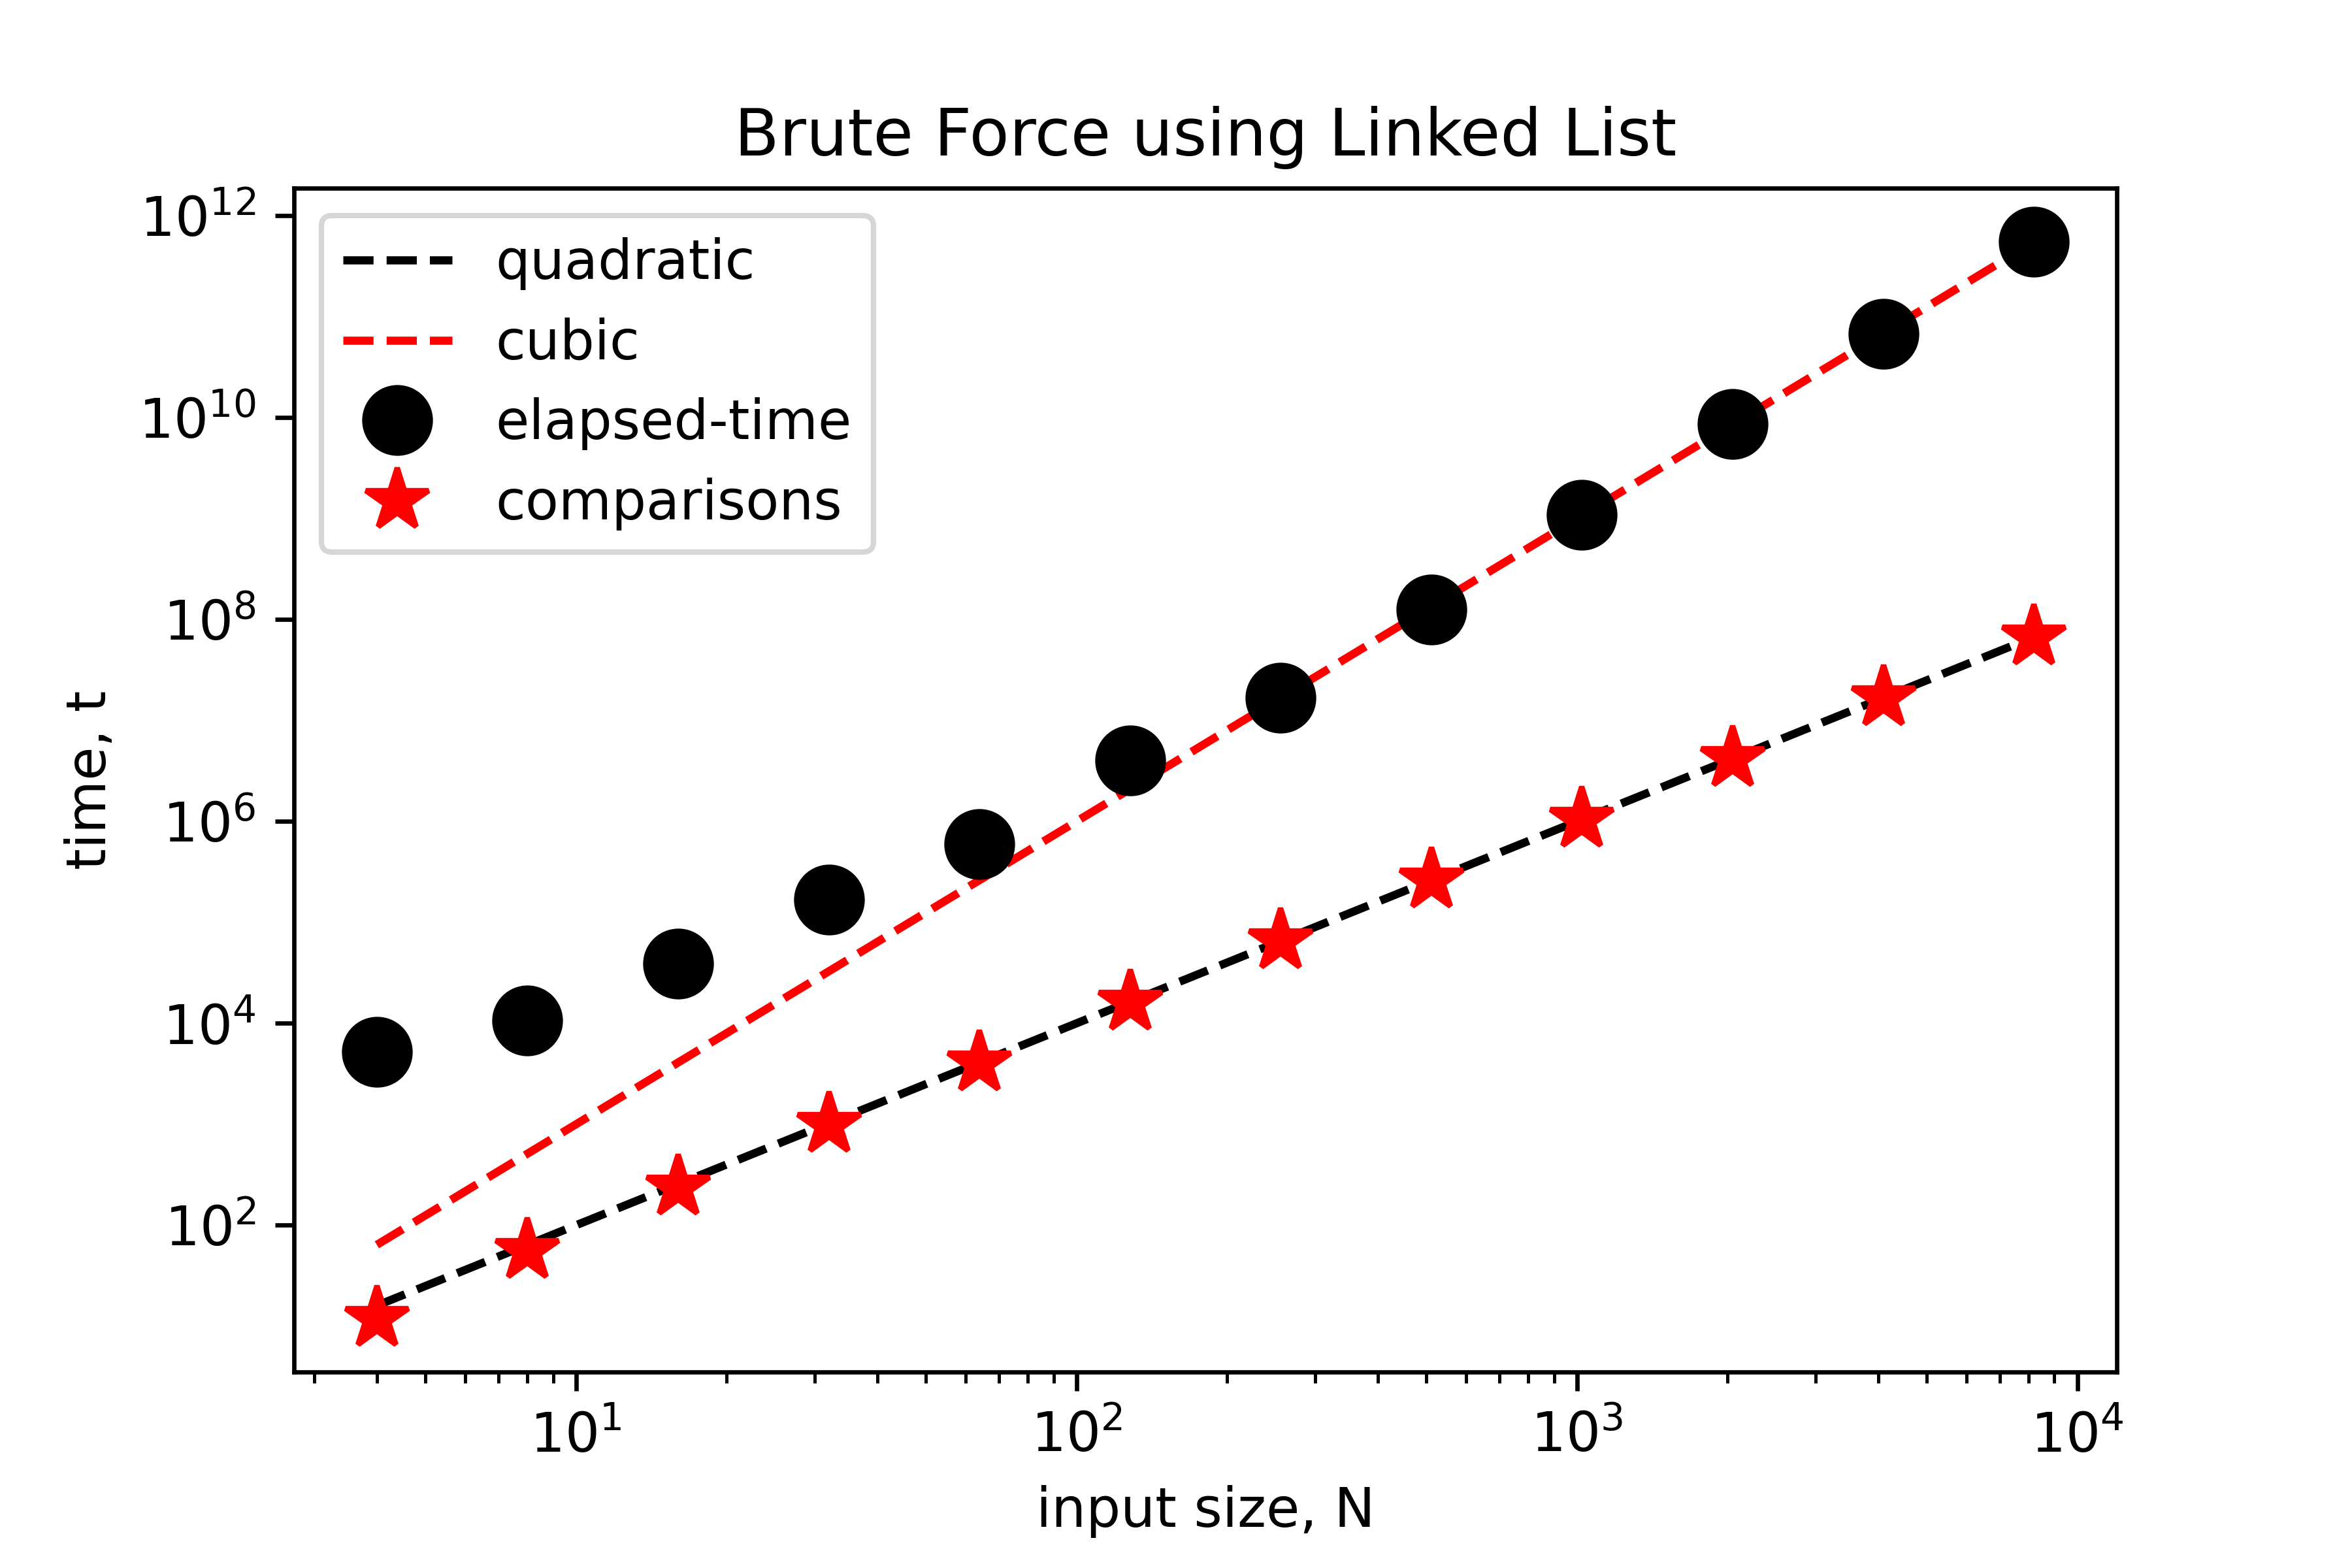
\includegraphics[width=0.45\textwidth,\keepaspectratio]{Images/BruteLinked.png}
    \caption{Comportamiento de la tecnica de \textit{Fuerza Bruta} usando \textit{Linked Lists}}
\end{figure}%

\begin{figure}[H]
    \centering    
    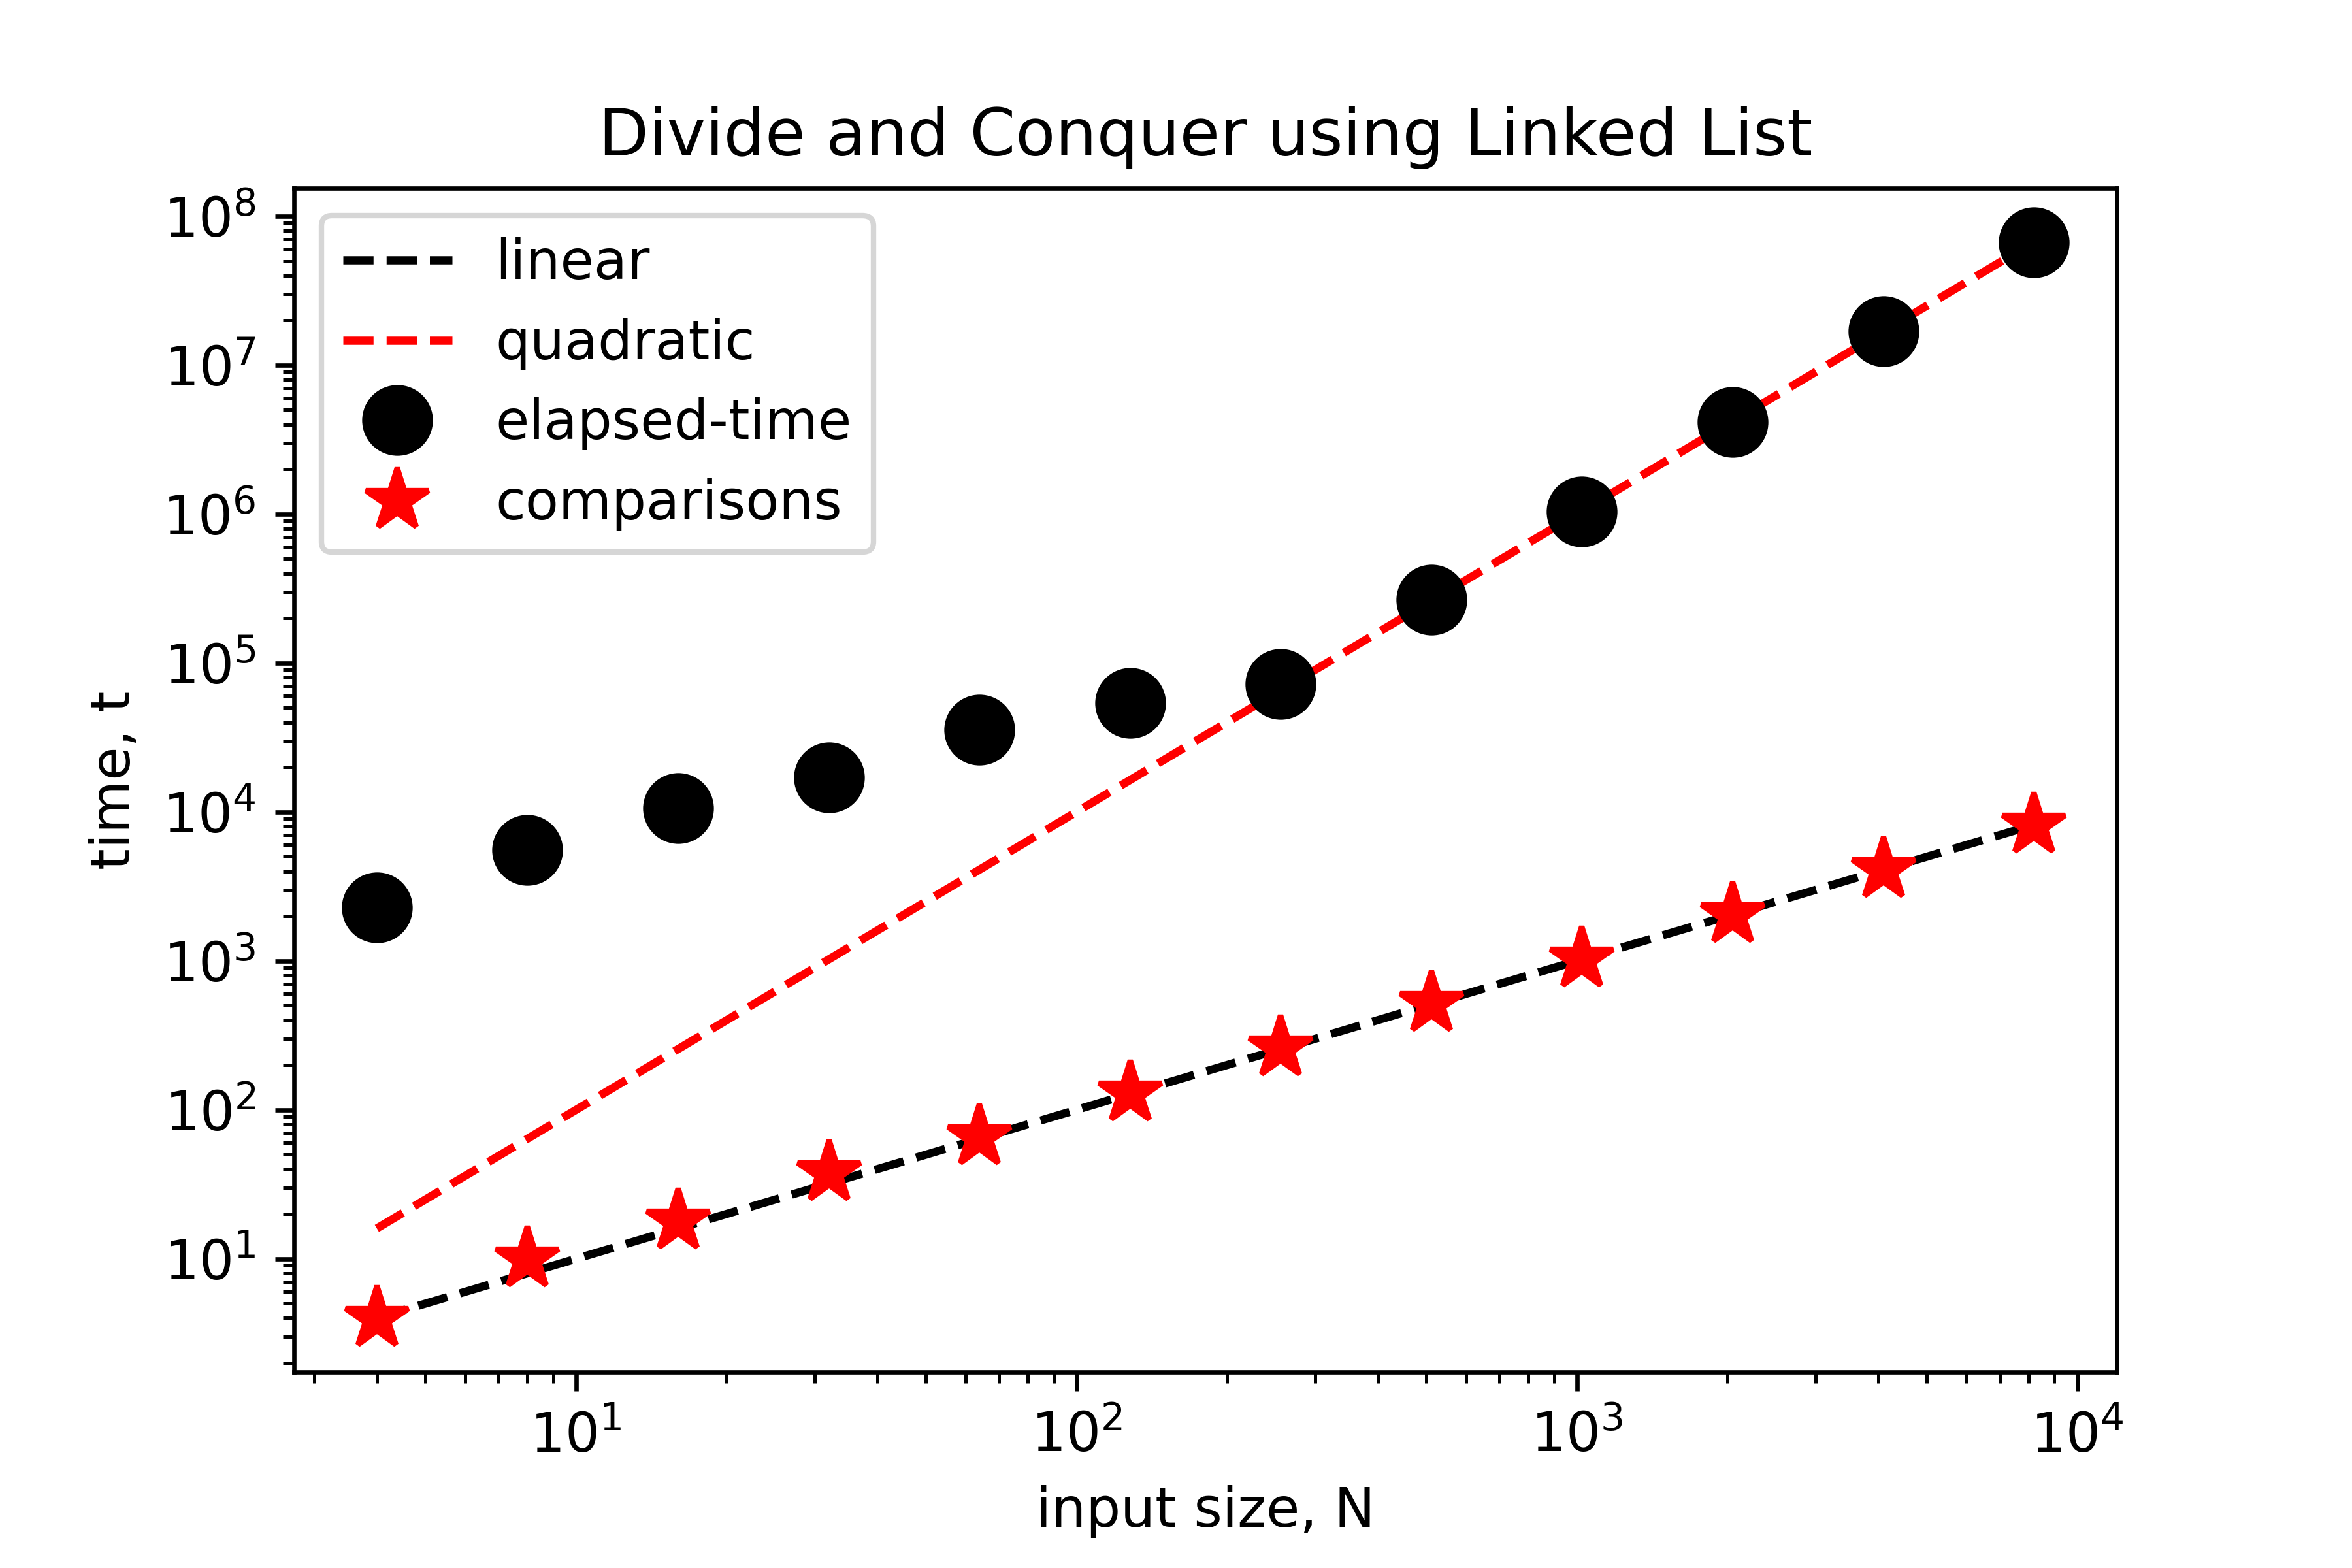
\includegraphics[width=0.45\textwidth,\keepaspectratio]{Images/DivideLinked.png}
    \caption{Comportamiento de la tecnica de \textit{Divide y Venceras} usando \textit{Linked Lists}}
\end{figure}%

Observando las gráficas podemos notar que usando la técnica de \textit{Divide y vencerás} el número de iteraciones crece de manera lineal $O(N)$ tanto para el método que usa \textit{Array Lists} como para el que usa \textit{Linked Lists}, aunque no de manera totalmente precisa, pues el número de iteraciones depende de la lista de coordenadas, por lo que los datos no están alineados en su totalidad al ajuste lineal, pero se comportan de manera parecida. Por otro lado, sin importar el tipo de estructura de datos que se use, el número de iteraciones de la técnica de \textit{Fuerza bruta} crece de manera exponencial $O(N^2)$, y sin importar los datos del arreglo el número de iteraciones dado un mismo N será el mismo y se ajusta de manera perfecta al ajuste exponencial. 
La diferencia está en que usando la técnica de \textit{Divide y vencerás}, el programa no compara cada par de puntos en la lista, sino que compara solo los que están más cercanos, lo que ahorra una gran cantidad de comparaciones y permite que el número de iteraciones aumenten de manera parecida a N, es decir de manera lineal. Mientras que usando la técnica de \textit{Fuerza bruta}, sin importar que las coordenadas estén muy lejanas se calcula la distancia entre ellas, lo que causa que se tengan que realizar muchas más comparaciones de las necesarias, y provocan que el número de iteraciones aumenten de manera exponencial a medida que aumente N.\\
Sin embargo, a pesar de que notamos que el crecimiento en el número de iteraciones dada la misma técnica de desarrollo de algoritmos se comporta de manera similar sin importar el tipo de estructura de datos, lo que si varia de manera significativa es la complejidad temporal, pues notamos que los tiempos de ejecución para los métodos que usaron \textit{Array Lists} fueron considerablemente menores que los tiempos de ejecución de los métodos que usaron \textit{Linked Lists}. Pues la complejidad temporal cuando se aplica la técnica de \textit{Divide y vencerás} usando \textit{Array Lists} es lineal $O(N)$, mientras que cuando se usan \textit{Linked Lists} la complejidad es cuadrática $O(N^2)$. Y cuando se aplica la técnica de \textit{Fuerza bruta} usando \textit{Array Lists} la complejidad temporal es cuadrática $O(N^2)$, mientras que cuando se usan \textit{Linked Lists} la complejidad es cubica $O(N^3)$. Esto es debido a que se puede acceder a los elementos de los \textit{Array Lists} directamente usando su \textit{index}, mientras que para los \textit{Array Lists} es necesario recorrer todos los elementos previos para acceder al elemento que se necesita. Por esta razón es que los métodos que usan \textit{Array Lists} son más rápidos que los que usan \textit{Linked Lists}.
